\section{Introduction}
Recent advances in biomedical image analysis have assisted many pathologists and biologists to facilitate their researches \cite{Chen2016b, Ronneberger2015,Chen2016c,Lieman-Sifry2017,Paszke2016,Tseng2017,Sirinukunwattana2015b}.
Among these researches, a significant application is to obtain the accurate segmentation of specific membrane objects in a biomedical image, such as lumenal glands, synaptic vesicles and cells.
Especially, the morphological shape and spatial distribution of synaptic vesicles are helpful to study the neural activity in different brain regions, while morphological statistics of lumenal glands are widely used for assessment of the malignancy degree of adenocarcinomas.
Conventionally, these crucial steps are performed by human expert, which are time-consuming and suffer from subjective factors.
Therefore, it is significantly demanded to improve the efficiency as well as the reliability with automatic segmentation methods.

\begin{figure}
    \begin{center}
        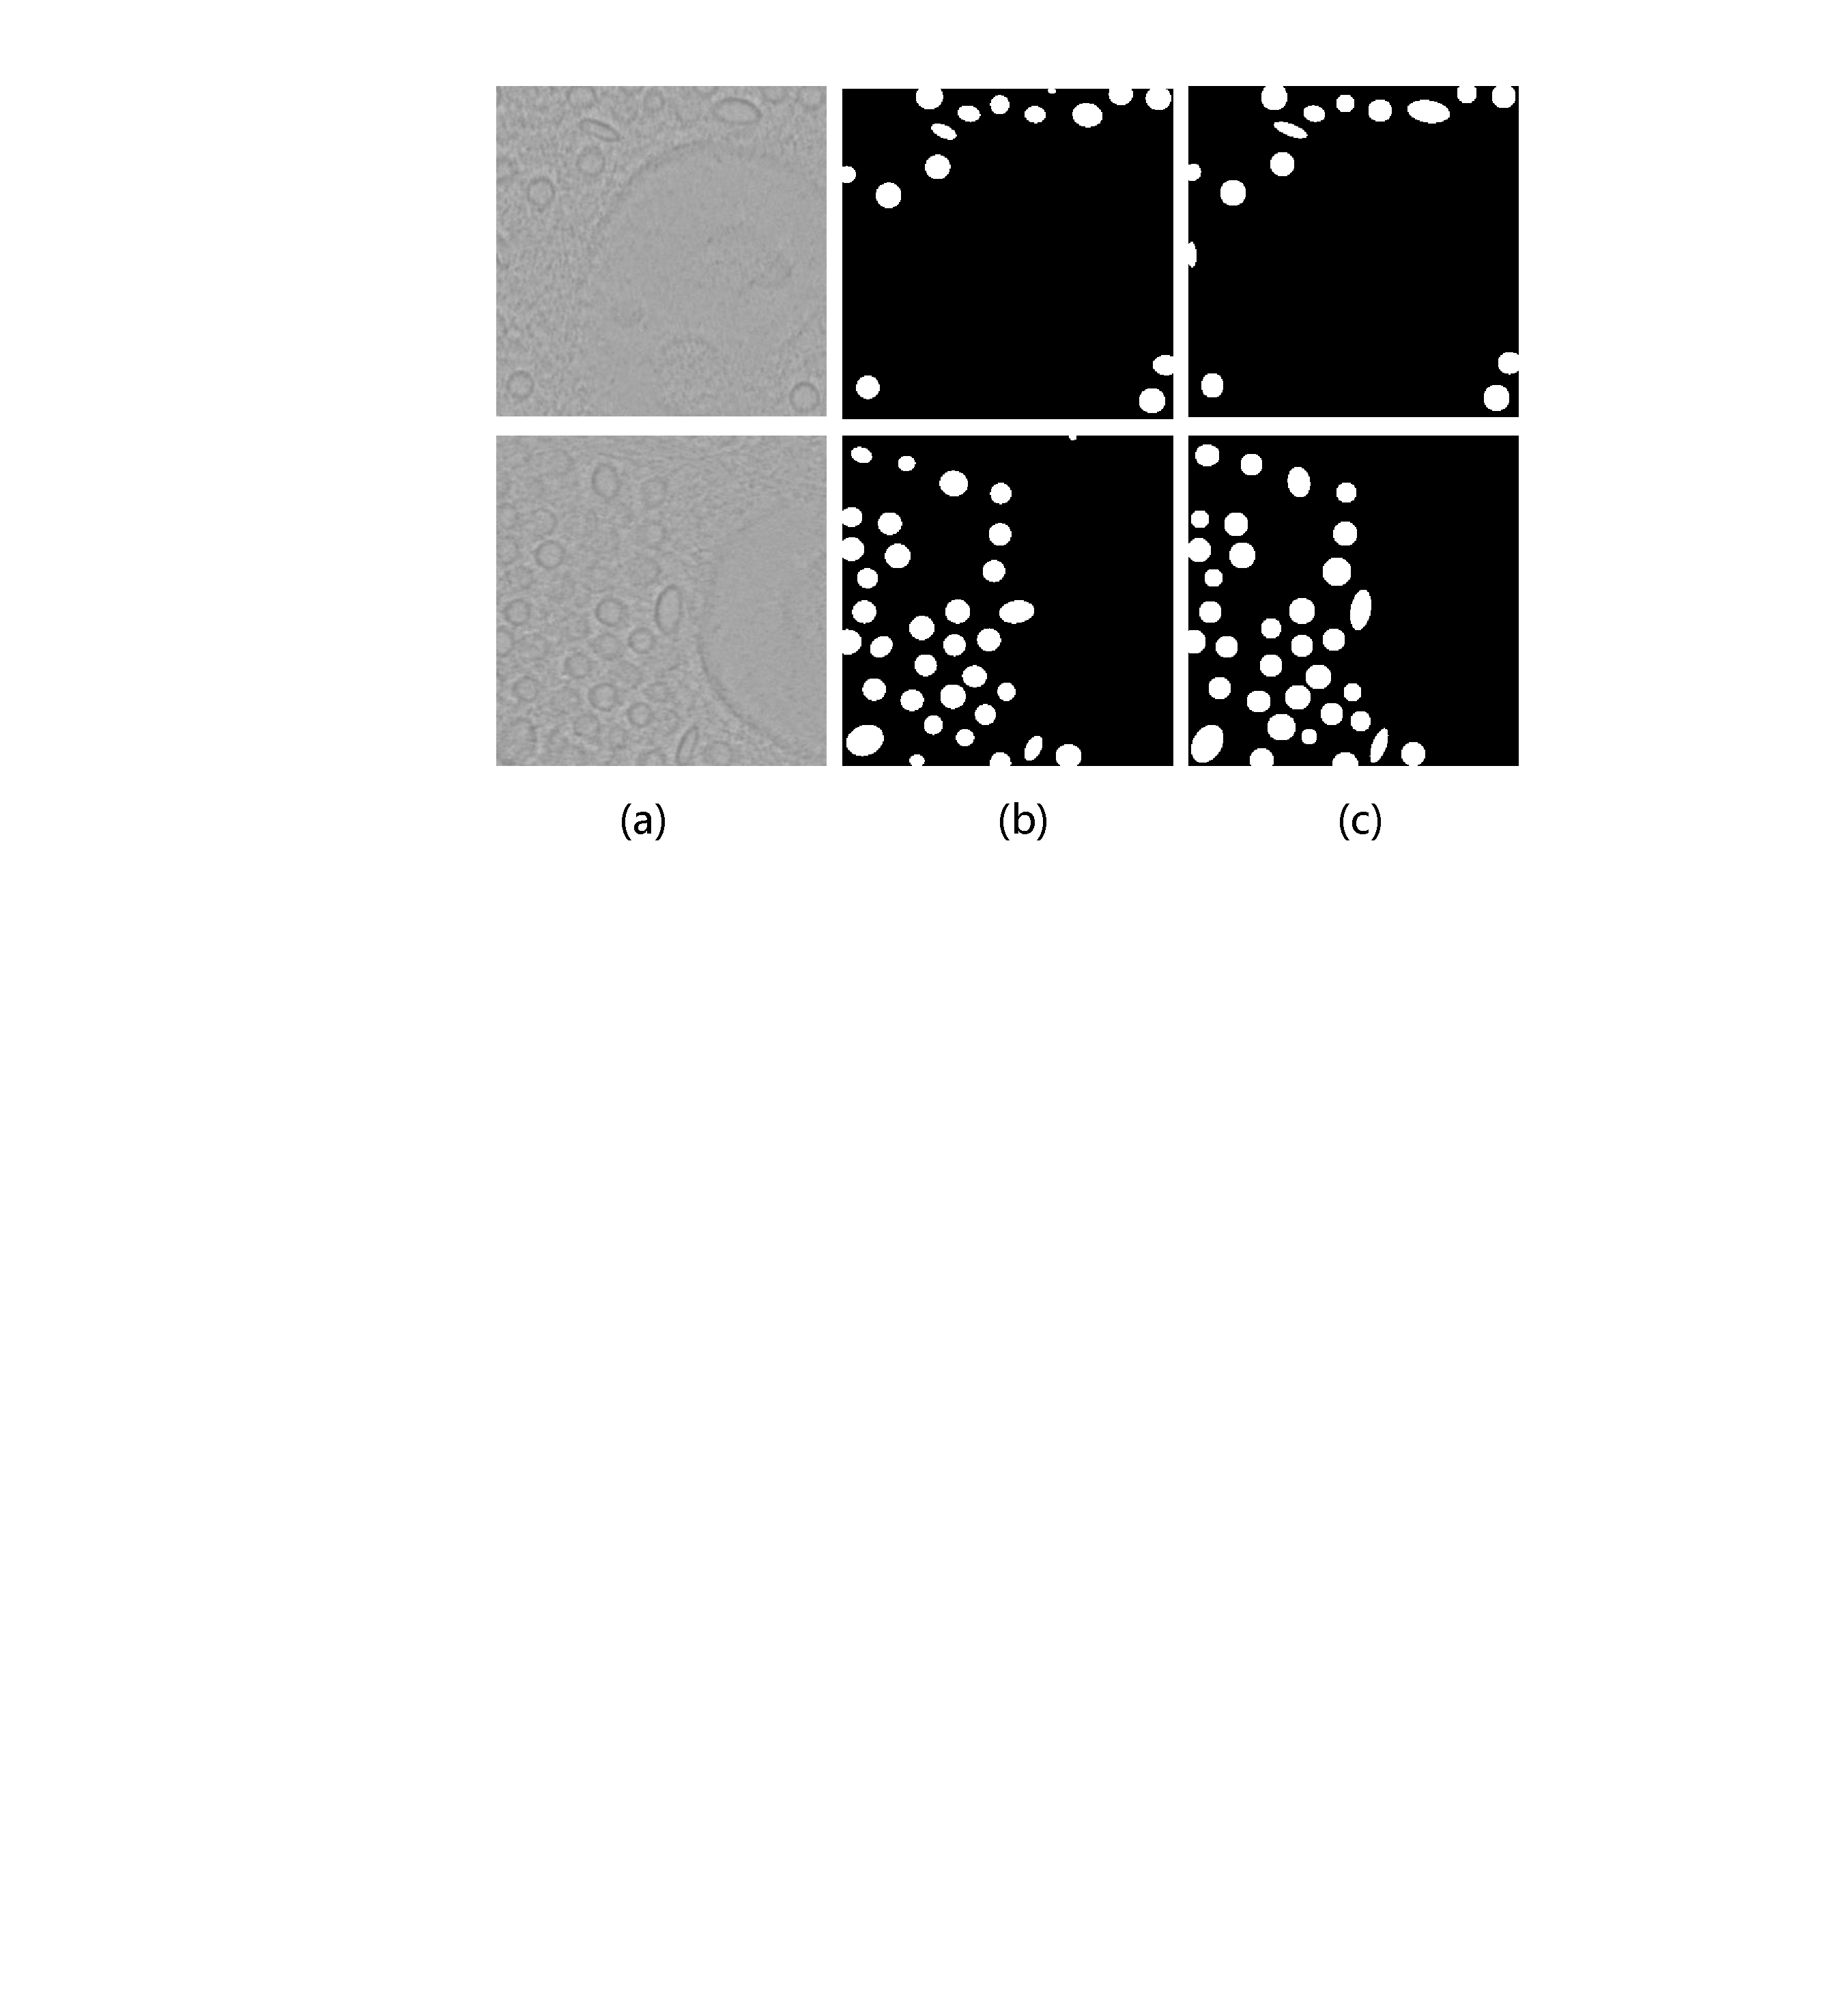
\includegraphics[width=3.3in]{figures/FigImg.pdf}
    \end{center}
    \caption{Examples of challenging biomedical segmentation: (a) biomedical image; (b) results from proposed DSAN by incorporating prior shape knowledge; (c) annotations by experts.}
    \label{FigImgs}
\end{figure}

However, it is non-trivial to automatically segment objects in biomedical images.
First, biomedical images are usually noisy and ambiguous caused by deficient imaging techniques, as shown in Figure~\ref{FigImgs} (a).
Second, as many plausible objects in biomedical images are densely arranged, it is hard to separate objects individually, which is known as the touching problem.
Third, although most objects in some biomedical image have regular shape, the prior shape knowledge is hard to to incorporated due to existing pathological cases with deformable shape\cite{Sirinukunwattana2015b}.

Recently, deep neural networks have demonstrated excellent performance in biomedical image segmentation with the use of fully convolutional networks (FCN) \cite{Dhungel2015,Ronneberger2015,Roth2015,Chen2015,Lieman-Sifry2017,Xu2016,Chen2016b}.
However, as the pooling and downsampling layers used in FCN usually make their localized object boundaries poor and coarse, the touching problem becomes serious.
To this end, many efforts have been made recently to increase the boundary accuracy.
An U-shaped deep network called U-net~\cite{Ronneberger2015} is proposed for biomedical image segmentation.
By employing the skip connections between contracting and expanding paths, context information can be directly propagated to higher resolution layers for detail preserving.
Several improvements of U-net were proposed soon afterwards.
For example, DeepVentricle~\cite{Lieman-Sifry2017}, which uses the same padding instead of valid padding, has been successfully used for cardiac segmentation.
Recently, DCAN~\cite{Chen2016a} integrates complementary information of objects and contours in a multi-task learning framework to separate the clustered objects into individual ones, which obtains the state of the art performance.
Although these methods achieved promising results in their segmentation tasks, they may fail to achieve satisfying performance in more blurry image with denser and smaller objects, which is more challenging for clear segmentation.

In this paper, we propose a first Deep Shape-Aware network (DSAN) to segment dense objects by inherently incorporating prior shape knowledge into network.
Similar with \cite{Chen2016a,Chen2016,Bertasius2016}, we formulate the network as a multi-task learning framework by simultaneously predicting an objectness score map and several auxiliary maps for an input image.
Instead of contour probability as auxiliary, our SCNN learns the parameterized expression of objects shape, which emphasizes more on the overall shape of objects.
Inspired by Region Proposal Network in \cite{Ren2015}, our SCNN simultaneously predicts an objectness score and a set of parameters, formulating the shape of a nearest object, at each pixel.
The complementary information in auxiliary parameters can not only separate the objects into individual ones, but also optimize their shapes.

However because of serious deformable objects in some pathological cases, the shape of objects cannot be parameterized uniformly and constrained strictly.
Therefore, we select a best representative shape as constraint and generate the final segmentation mask using a piecewise fusion strategy to achieve a balance between regularization and unconstraint for each object.
Furthermore, a novel split max pooling (SMP) is proposed to improve both objectness scores and shape parameters by exploring the intrinsic correlation between them for better results.
Especially, SMP is designed as a trainable layer, which can be trained end-to-end and easily extended to any multi-task networks.
In this way, our DSAN can not only optimize the segmented shape of regular objects with prior shape knowledge, but also accommodates seriously deformable objects.

Overall, the contribution of this paper is three-fold:
\begin{enumerate}
	\item We first effectively incorporate shape constraint into deep neural networks.
	% for biomedical image segmentation.
	\item We propose a novel split max pooling for benefiting both multi-task outputs.
	\item Our framework is applicable to a series of different tasks such as biomedical image segmentation, scent detection task and achieves the state-of-the-art performance.
\end{enumerate}
